\title{\textsc{Corn}}
\author{Giorgio Giuffr\`e \\ 1069456}
\date{}

\documentclass[12pt]{article}
\usepackage[utf8]{inputenc}
\usepackage{mathtools}
\usepackage{amssymb}
\usepackage{tikz}
\usepackage{tkz-graph}
\renewcommand*{\EdgeLineWidth}{0.15pt}

\tikzset{
	every neuron/.style={
		circle,
		draw,
		minimum size=1cm
	},
	neuron missing/.style={
		draw=none, 
		scale=4,
		text height=0.333cm,
		execute at begin node=\color{black}$\vdots$
	},
}



\begin{document}
\maketitle



%%% ========================================
%%% ========================================

\begin{abstract}
\textsc{Corn} (COstruttore di Reti Neurali) è una piccola piattaforma che permette di progettare e allenare semplici reti neurali artificiali feedforward (cioè acicliche), per poi collaudarle su input numerici.
\end{abstract}



%%% ========================================
%%% ========================================

\section{Introduzione}

\subsection{Cos'è una rete neurale?}

\paragraph{}
Il miglior esempio di rete neurale è senza dubbio il cervello umano: una rete di cellule collegate tra loro --- dette neuroni --- alcune delle quali si interfacciano con l'ambiente esterno (i neuroni sensoriali e i neuroni motori) mentre altre stanno “nascoste” all'interno, nei meandri della rete. Ciò che succede nel cervello è apparentemente caotico: ogni neurone manda un segnale a più neuroni e riceve segnali da neuroni diversi, determinando un'intricata catena parallela di segnali che termina con i neuroni motori, collegati ai muscoli delle gambe, della bocca, delle mani eccetera. Eppure, questa architettura intricata è alla base del pensiero e del comportamento umano.

\paragraph{}
Con un po' di fantasia, possiamo vedere i neuroni di input e di ouput (detti neuroni “visibili”) come l'\textit{interfaccia} della rete con l'utente, mentre i neuroni nascosti costituiscono l'\textit{implementazione} di un certo algoritmo.

\paragraph{}
In poche parole, una rete neurale è un grafo orientato in cui ogni nodo è un \textbf{neurone} e ogni arco è un \textbf{collegamento} che va da un neurone a un altro. Un neurone è una cellula che riceve uno o più segnali di input, li somma ed emette un solo segnale di output (quindi è una funzione $f : \mathbb{R}^n \rightarrow \mathbb{R}$, dove $n \ge 1$ è il numero di segnali in ingresso). In base al segnale totale di input $x$, ogni neurone emette quindi un certo segnale di output $f(x)$ che può poi ramificarsi, cioè può essere mandato a più di un neurone, a seconda di com'è disegnato il grafo. Le connessioni (gli archi) tra un neurone e l'altro sono pesate, cioè ogni input $x_i$ viene moltiplicato per una costante reale $w_i$ che può essere modificata dalla rete nel corso del tempo.

\paragraph{}
Tutti i neuroni della rete implementano la stessa semplice funzione $f$, detta \textbf{funzione di attivazione}. Chiaramente, l'output di due neuroni può essere diverso, per il fatto che gli archi della rete non hanno tutti lo stesso peso. La capacità della rete di modificare i pesi delle proprie connessioni fa sì che essa sia capace di associare ad ogni input un certo output desiderato. Ad esempio, una rete con due neuroni di input e un neurone di output può modificare i propri pesi in modo da imparare a calcolare la media di due numeri che le vengono presentati:

\begin{center}
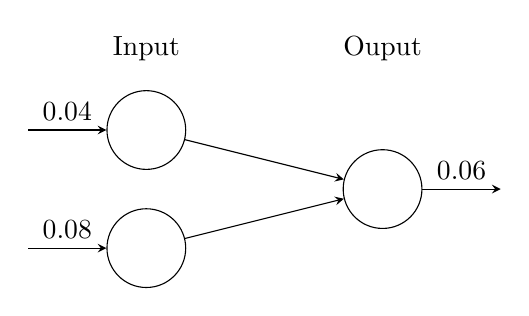
\begin{tikzpicture}[x=1.5cm, y=1.5cm, >=stealth]

\foreach \m/\l [count=\y] in {1,2}
	\node [every neuron/.try, neuron \m/.try] (input-\m) at (0,2-\y) {};

\foreach \m [count=\y] in {1}
	\node [every neuron/.try, neuron \m/.try ] (output-\m) at (2,1.5-\y) {};

\foreach \l [count=\i] in {0.04, 0.08}
	\draw [<-] (input-\i) -- ++(-1,0)
		node [above, midway] {$\l$};

\foreach \l [count=\i] in {0.06}
	\draw [->] (output-\i) -- ++(1,0)
		node [above, midway] {$\l$};

\foreach \i in {1,2}
	\foreach \j in {1}
		\draw [->] (input-\i) -- (output-\j);

\foreach \l [count=\x from 0] in {Input, Ouput}
  \node [align=center, above] at (\x*2,1.5) {\l};

\end{tikzpicture}
\end{center}

La rete apprende grazie ad una serie di \textbf{esempi} che le vengono presentati: $(0.04, 0.08 \rightarrow 0.06)$, $(0.05, 0.01 \rightarrow 0.03)$, $(0.02, 0.05 \rightarrow 0.035)$, $(0.09, 0.08 \rightarrow 0.085)$ e così via. Più esempi vengono forniti, più è preciso l'apprendimento. A questo proposito, è importante notare che la rete fornisce risposte \textit{approssimate}, dovendo imparare da un insieme di esempi anziché da delle regole esplicite.

\paragraph{}
Oppure, una rete con 4 neuroni in ingresso e 4 in uscita (con un livello di neuroni nascosti) potrebbe imparare a calcolare il successore di un numero in formato binario\footnote{I pallini neri nel disegno indicano la presenza di eventuali altre neuroni nascosti, oltre ai due disegnati}:

\begin{center}
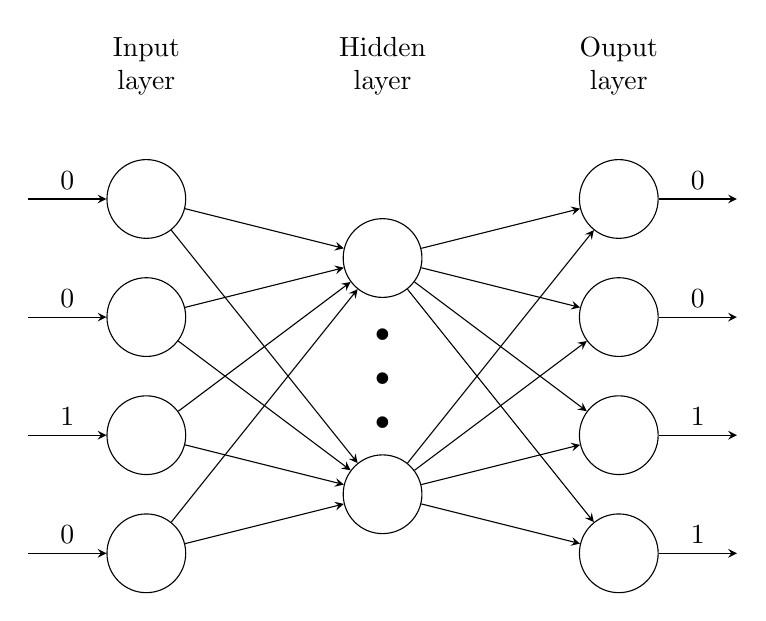
\begin{tikzpicture}[x=1.5cm, y=1.5cm, >=stealth]

\foreach \m/\l [count=\y] in {1,2,3,4}
	\node [every neuron/.try, neuron \m/.try] (input-\m) at (0,2-\y) {};

\foreach \m/\l [count=\y] in {1,missing,2}
	\node [every neuron/.try, neuron \m/.try] (hidden-\m) at (2,1.5-\y) {};

\foreach \m [count=\y] in {1,2,3,4}
	\node [every neuron/.try, neuron \m/.try ] (output-\m) at (4,2-\y) {};

\foreach \l [count=\i] in {0,0,1,0}
	\draw [<-] (input-\i) -- ++(-1,0)
		node [above, midway] {$\l$};

\foreach \l [count=\i] in {0,0,1,1}
	\draw [->] (output-\i) -- ++(1,0)
		node [above, midway] {$\l$};

\foreach \i in {1,...,4}
	\foreach \j in {1,...,2}
		\draw [->] (input-\i) -- (hidden-\j);

\foreach \i in {1,...,2}
	\foreach \j in {1,...,4}
		\draw [->] (hidden-\i) -- (output-\j);

\foreach \l [count=\x from 0] in {Input, Hidden, Ouput}
  \node [align=center, above] at (\x*2,1.8) {\l \\ layer};

\end{tikzpicture}
\end{center}

\subsection{Cosa può fare \textsc{Corn}?}

\paragraph{}
Insomma, i compiti che una rete può imparare sono numerosissimi e \textsc{Corn} offre un'interfaccia semplice per specificare sia la configurazione della rete sia i compiti da farle imparare. La progettazione di una rete neurale artificiale si articola in tre fasi: Definizione dell'architettura della rete; definizione degli esempi da presentare alla rete; allenamento della rete. Una volta allenata la rete, la si può interrogare su degli input numerici.



%%% ========================================
%%% ========================================

\section{Guida all'uso}

\paragraph{}
\textsc{Corn} consiste di una sola finestra principale, dalla quale l'utente può lavorare su una rete alla volta. La finestra principale presenta, a sinistra, un elenco delle rete finora create (oltre a quelle disponibili di default); basta cliccare su una rete dell'elenco per potersi interfacciare con essa.

\paragraph{}
Come detto prima, la progettazione di una rete si articola in tre semplici fasi:
\begin{itemize}
	\item definizione dell'architettura della rete;
	\item definizione degli esempi su cui la rete si allenerà;
	\item allenamento vero e proprio.
\end{itemize}
La prima cosa da fare, quindi, è andare sul menù “Rete” e cliccare “Nuova Rete”. La finestra principale contiene ora un pannello dal quale possiamo costruire la rete. Innanzitutto bisogna decidere il \textbf{nome} con cui battezzare la rete (senza l'estensione \textit{.net}, aggiunta automaticamente); è utile darle il nome del compito che deve imparare: ad esempio, una rete che debba apprendere a calcolare la somma tra quattro numeri potrebbe chiamarsi “sum\_4”, per poterla ritrovare poi con più facilità. Si deve poi selezionare il \textbf{tipo di funzione di attivazione} dei neuroni (la stessa funzione per tutti i neuroni: ciò che cambia sono solo i pesi delle connessioni) e infine il \textbf{numero di livelli} della rete (includendo nel conto il livello di input e quello di output). Più il compito è elaborato, più livelli ci vogliono; generalmente, uno o due livelli nascosti vanno più che bene ma, se l'utente vuole sperimentare, può selezionare fino a 8 livelli. Cliccando “Prosegui...”, l'utente potrà poi specificare il \textbf{numero di neuroni} per ogni livello; i livelli sono ordinati dall'input all'output e i più importanti sono il primo e l'ultimo, che dovranno contenere rispettivamente il numero di neuroni in ingresso e il numero di neuroni in uscita. Ora, basta cliccare “Crea” e la nuova rete comparirà nell'elenco delle reti, a sinistra nella finestra principale.

\paragraph{}
Per scrivere gli esempi da presentare alla rete, dal menù “Dati” bisogna selezionare “Nuovo foglio di esempi”. Quello che viene presentato all'utente è un editor di testo diviso in due parti: nella prima va inserito l'input del singolo esempio; nella seconda l'output desiderato. Ogni esempio va aggiunto con “Aggiungi” e dopo aver aggiunto l'ultimo basta cliccare “Crea” e rispondere alla finestra di dialogo indicando il nome del foglio di esempi (senza l'estensione \textit{.data}). Ancora, è opportuno dare il nome del compito da imparare: un foglio di esempi per la media tra due numeri si può intitolare “avg\_2” o “media”.

\paragraph{}
Dobbiamo ora allenare la nostra rete --- i cui pesi sono inizializzati in modo casuale --- sul foglio di esempi appena creato. Per fare ciò clicchiamo navighiamo nell'elenco di reti a sinistra fino a trovare la rete che cerchiamo. Si apre ora l'interfaccia utente-rete, dalla quale possiamo scegliere se allenare la rete o interrogarla su degli input: basta scegliere tra le due tab in alto. Può essere interessante collaudare la rete prima ancora di averla allenata: darà degli output insensati per via del fatto che i pesi delle sue connessioni sono stati inizializzati a caso.
Per allenarla, invece, selezioniamo il foglio di dati appropriato ... ...



%%% ========================================
%%% ========================================

\section{Implementazione}

\paragraph{}
Il programma è stato progettato seguendo lo schema \textit{Model View}. L'utente si interfaccia con una sola finestra principale, che cambia apparenza durante le varie fasi della progettazione di una rete neurale. Le reti neurali progettate (o quelle già disponibili come esempi) sono controllate da una classe “Model” ...

\subsection{Parte logica}

\begin{center}
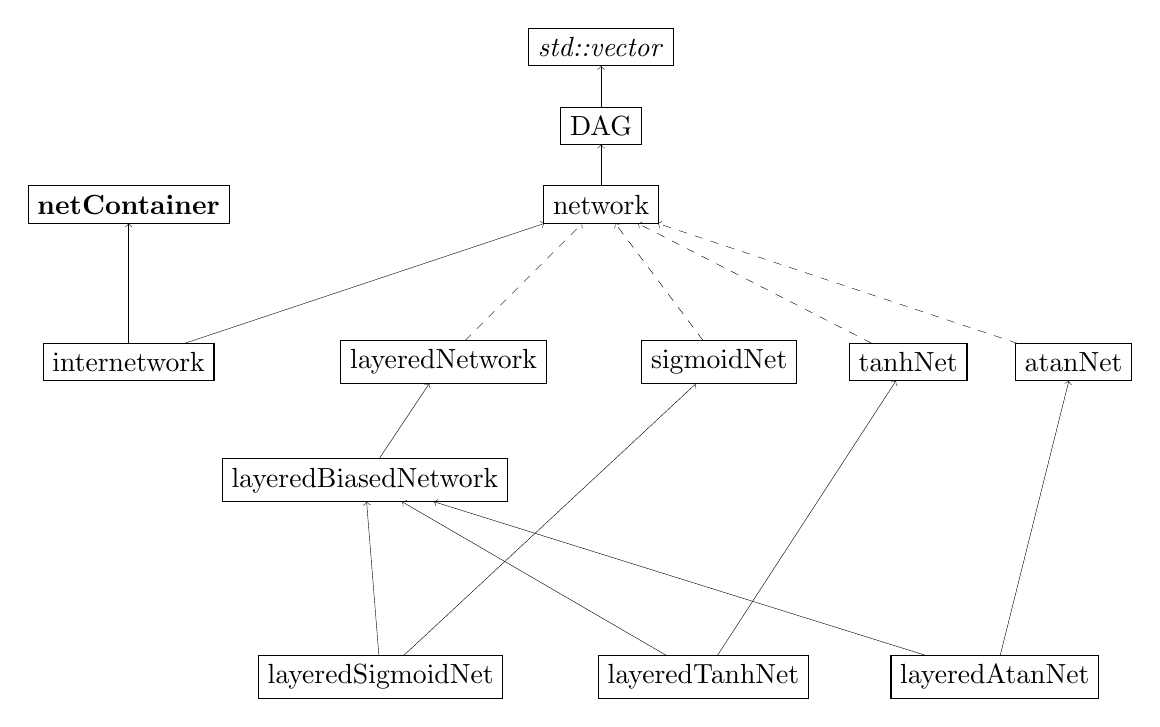
\begin{tikzpicture}
\tikzset{VertexStyle/.style = {shape=rectangle, fill=white, draw}}
\tikzset{EdgeStyle/.style = {->}}

\Vertex[L=\textit{std::vector}]{vector}
	\Vertex[x=0,y=-1]{DAG}
		\Vertex[x=0,y=-2]{network}
			\Vertex[x=-2,y=-4]{layeredNetwork}
				\Vertex[x=-3,y=-5.5]{layeredBiasedNetwork}
			\Vertex[x=1.5,y=-4]{sigmoidNet}
			\Vertex[x=3.9,y=-4]{tanhNet}
			\Vertex[x=6,y=-4]{atanNet}

					\Vertex[x=-2.8,y=-8]{layeredSigmoidNet}
					\Vertex[x=1.3,y=-8]{layeredTanhNet}
					\Vertex[x=5,y=-8]{layeredAtanNet}

					\Vertex[x=-6,y=-4]{internetwork}

		\Vertex[x=-6,y=-2,L=\textbf{netContainer}]{netContainer}

\Edge(DAG)(vector)
\Edge(network)(DAG)
\Edge[style={dashed}](layeredNetwork)(network)
\Edge(layeredBiasedNetwork)(layeredNetwork)
\Edge[style={dashed}](sigmoidNet)(network)
\Edge[style={dashed}](tanhNet)(network)
\Edge[style={dashed}](atanNet)(network)
\Edge(layeredSigmoidNet)(sigmoidNet)
\Edge(layeredSigmoidNet)(layeredBiasedNetwork)
\Edge(layeredTanhNet)(tanhNet)
\Edge(layeredTanhNet)(layeredBiasedNetwork)
\Edge(layeredAtanNet)(atanNet)
\Edge(layeredAtanNet)(layeredBiasedNetwork)
\Edge(internetwork)(network)
\Edge(internetwork)(netContainer)
\end{tikzpicture}
\end{center}

\subsection{Interfaccia grafica}

...



\end{document}
